\documentclass[10pt, aspectratio = 169]{beamer}
% Use package form https://github.com/tgodfrey0/soton-beamer/tree/main
% Theme choice
\usetheme{Soton}
\usecolortheme{default}

% Title page information
\title{Machine Learning with graphs - Project Defense}
\subtitle{Delaunay Graph: Addressing Over-Squashing and Over-Smoothing Using
Delaunay Triangulation\\
by Attali H., Duscaldi D. and Pernelle N. \texorpdfstring{\cite{attali2024delaunay}}}

\author{Edwin Roussin and Tristan Waddington}
\supervisor{Supervised by Jhony H. Giraldo}
\institute{IP-Paris, CEMST}
\date{26/03/2025}

\setTitleLogoRight{figures/CEMS Terre_nouveau logo792x445px.png}
% \setTitleLogoCentre{robot.pdf}
\setTitleLogoLeft{figures/ipparis.png}
\setLogo{figures/ipparis.png}
% \setColourScheme{50}{85}{234}
% \setProgressBarOff
% \setFrameNumbersOff

\begin{document}

% Title slide
\begin{frame}
    \titlepage
\end{frame}

% Introduction
\begin{frame}
    \frametitle{Introduction}
    \begin{block}{Delauney triangulation}
    Reconstruct a graph completely from projected features using the Delaunay triangulation.

    $\Rightarrow$ Avoid \textbf{over-smoothing} and \textbf{over-squashing}.
    \end{block}
    
    \begin{figure}
        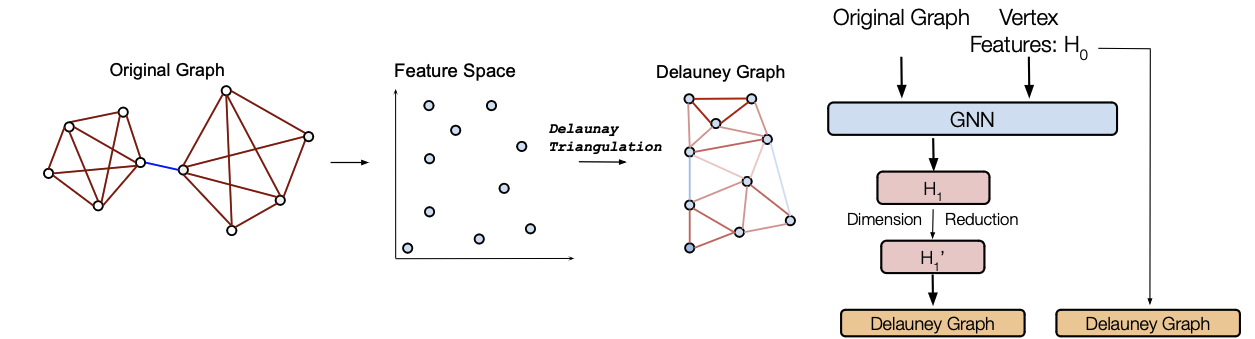
\includegraphics[width=0.7\textwidth]{figures/Delaunay-Rewiring.png}
        \caption{Illustration of the Delaunay rewiring \cite[Attali al., 2024]{attali2024delaunay}}
    \end{figure}
\end{frame}


% Automatic Outline slide
\begin{frame}
    \frametitle{Outline}
    \tableofcontents
\end{frame}

% =====================================
% Need of graph rewiring
% =====================================
\section{Need of graph rewiring}

\subsection{Over-Squashing}
\begin{frame}
    \frametitle{Over-Squashing: inefficient information propagation}
    
    \begin{columns}
        \begin{column}{0.4\textwidth}
            \begin{figure}
                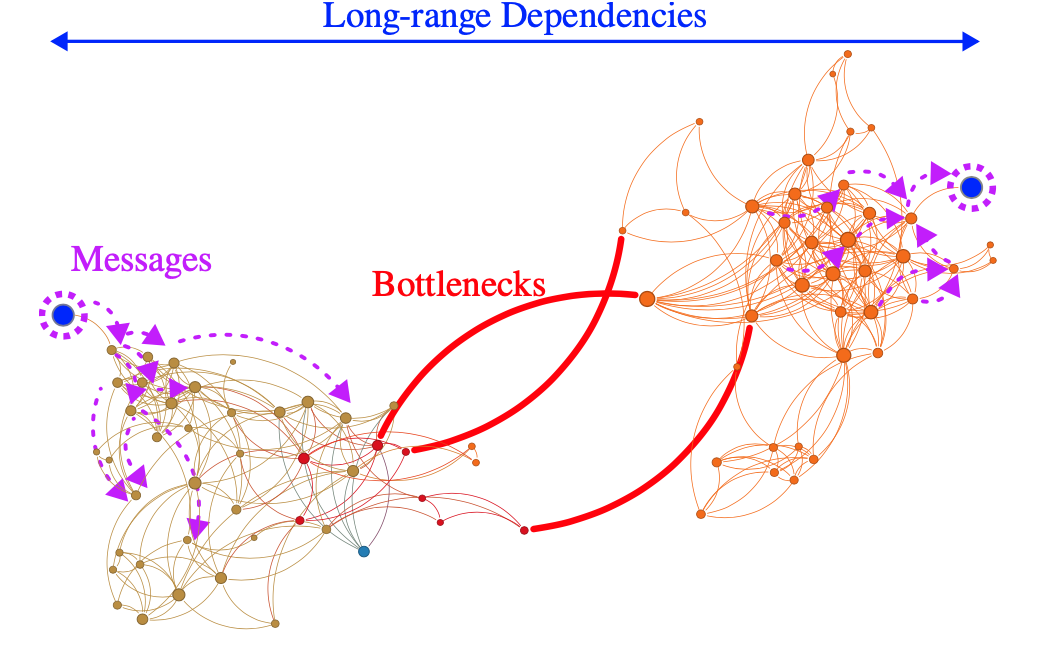
\includegraphics[width=0.99\textwidth]{figures/over_squashing_Girarldo.png}
                \caption{Illustration of Bottlenecks [Giraldo, Lecture GNNs, 2025]}
            \end{figure}

        \end{column}    
        \begin{column}{0.6\textwidth}
            GNNs struggle to propagate info to distant nodes: \textbf{bottleneck} 
            when aggregating messages across a long path \cite[Alon et al., 2021]{alon2021bottleneckgraphneuralnetworks}.
            
            Causes \textbf{over-squashing} of exponentially growing info into fixed-size vectors.
            $\Rightarrow$ \emph{Perform poorly when prediction task depends on long-range interaction.}

            \begin{block}{Vulnerable GNNs}
                GNC and GIN \emph{absorb incoming edges equally}, more susceptible to over-squashing than GAT and GGNN.
            \end{block}
            \begin{block}{Curvature metric}
                \emph{Discrete Ricci curvature} \cite[Topping et al. 2021]{topping2022understandingoversquashingbottlenecksgraphs} to identify bottlenecks.
            \end{block}
        \end{column}
    \end{columns}
\end{frame}

\subsection{Over-Smoothing}
\begin{frame}
    \frametitle{Over-Smoothing: consequence of message passing paradigm}
    \begin{columns}
        \begin{column}{0.6\textwidth}
            \begin{block}{Message-passing neural networks (MPNN):}
                Iterative approach, updating node representations through 
            the local aggregation of information from neighboring nodes.
            \end{block}
            Causes \textbf{over-smoothing} by the need to stack additional layers to capture non-local interactions.
            Will smooth-out heterophilic graphs.
            $\Rightarrow$ \emph{Nodes' representations are similar.}
        \end{column}
        \begin{column}{0.4\textwidth}
            \begin{figure}
                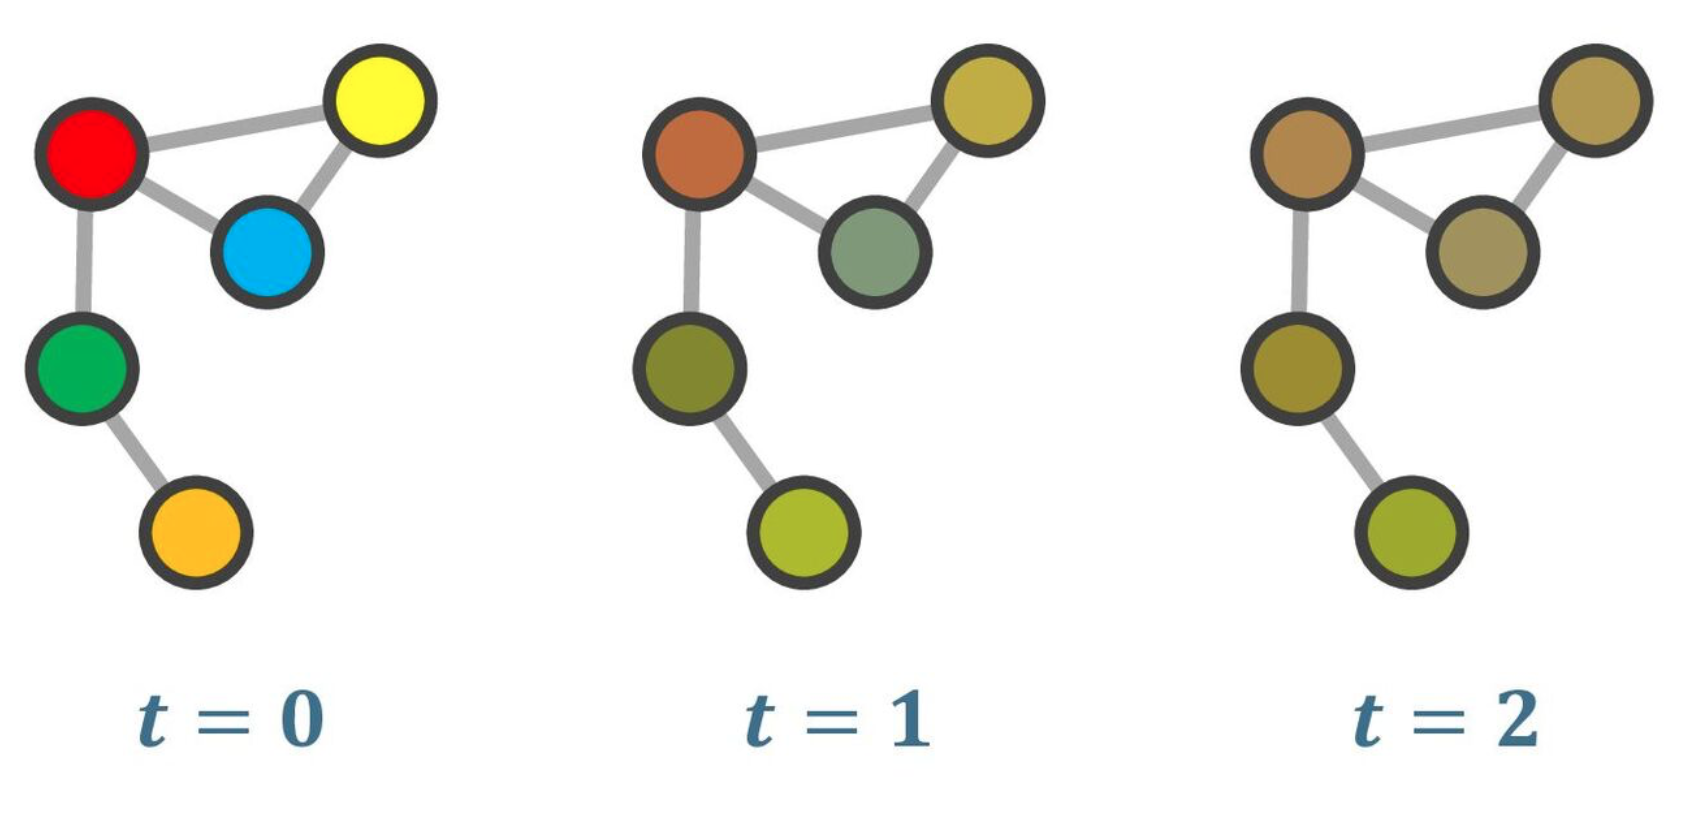
\includegraphics[width=0.99\textwidth]{figures/over_smoothing.png}
                \caption{Illustration of Over-smoothing by 
                \href{https://speakerdeck.com/utf/a-gentle-introduction-to-graph-neural-networks?slide=29}{Alex Ganose}}
            \end{figure}
        \end{column}
    \end{columns}
\end{frame}

\subsection{Existing solutions}
\begin{frame}
    \frametitle{Existing solutions}
    \textbf{Identify the quality of the message passing}:
    \begin{itemize}
        \item \textbf{Graph structure analysis} using curvature, but does not scale.
        \\Highly positive curved edges $\rightarrow$ over-smoothing \cite[Nguyen et al., 2023]{nguyen2023revisiting}.
        \\Highly negative curved edges $\rightarrow$ over-squashing \cite[Topping et al., 2021]{topping2022understandingoversquashingbottlenecksgraphs}.
        \item \textbf{Need original graph} but sometimes only features available (NER, documents, ...).
    \end{itemize}

    \textbf{Avoid over-smoothing in preventing the embedding to become the same}:
    \begin{itemize}
        \item \textbf{Normalization} with PairNorm \cite[Zaho, 2020]{zhao2020pairnorm}.
        \item \textbf{Rewiring} Drop edges, at random \cite[Rong, 2019]{rong2019dropedge} 
              or in finding the potential good ones \cite[Giraldo, 2023]{Giraldo_2023}
    \end{itemize}

    \begin{alertblock}{Over-smoothing and over-squashing are intrinsically related}
        Inevitable trade-off between these two issues, as they cannot be alleviated simultaneously.
        Quadratic complexity in the number of nodes (or edges).
    \end{alertblock}

\end{frame}

% =====================================
% Key technical novelty of the paper
% =====================================
\section{Key technical novelty of the paper}

\subsection{Theoretical Analysis}


\begin{frame}
    \frametitle{Theoretical analysis}
    \begin{columns}
        \begin{column}{0.6\textwidth}
        \begin{block}{Delaunay rewiring}
            Is an extreme \textbf{4 steps rewiring} method.
            \begin{enumerate}
                \item First GNN\footnote{GCN from \cite[Kipf and Welling, 2017]{kipf2017semi}} construct \textbf{node embeddings}   .
                \item Reduce the embedding with \textbf{UMAP} in dim 2.
                \item \textbf{Rebuilt edges with Delaunay triangulation}.
                \item Second GNN \textbf{mix with the original features} of the graph.
            \end{enumerate}

        \end{block}
        \end{column}
        \begin{column}{0.4\textwidth}
            \begin{figure}
                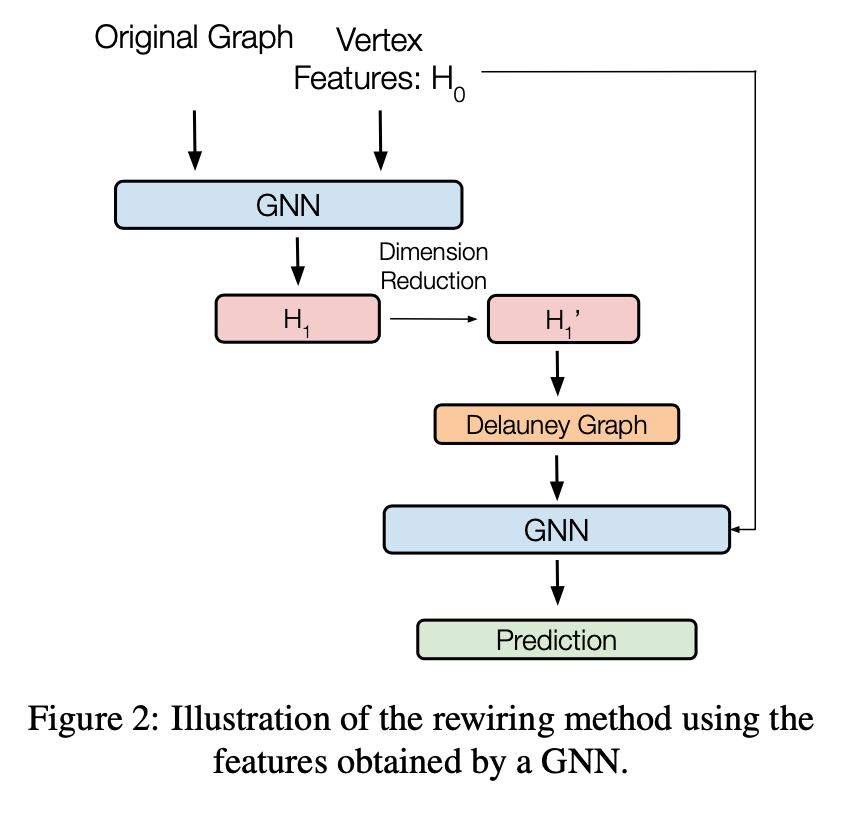
\includegraphics[width=0.99\textwidth]{figures/Rewiring_method.png}
                %\caption{Illustration of the Delaunay [Attali al., 2024] \cite{attali2024delaunay}}
            \end{figure}
        \end{column}
    \end{columns}
\end{frame}

\begin{frame}
    \frametitle{Initial Thoughts}
    \begin{columns}
        \begin{column}{0.5\textwidth}
            \begin{block}{Simplicity of the Method}
                No hyper-parameters = no grid-search. 
                Complexity of $\mathcal{O} \big( N \log N \big)$
            \end{block}
            \begin{block}{Graph creation method}
                Create a graph from the embedding $\Rightarrow$ no need for the original graph.
            \end{block}
        \end{column}
        \begin{column}{0.5\textwidth}
            \begin{alertblock}{Umap in 2 dimensions only}
                Triangulation in higher dimensions $\Rightarrow$ longer time + denser resulting 
                graphs~\footnote{Generalized triangles in dim=3: have 6 edges, 10 in dim=4} + worse accuracy.
            \end{alertblock}
            \begin{alertblock}{First GNN}
                Embed the initial smoothing and squashing? But needed for quality of 
                embedding. Long range dependencies? 
            \end{alertblock}
        \end{column}
    \end{columns}
    % \begin{figure}
    %     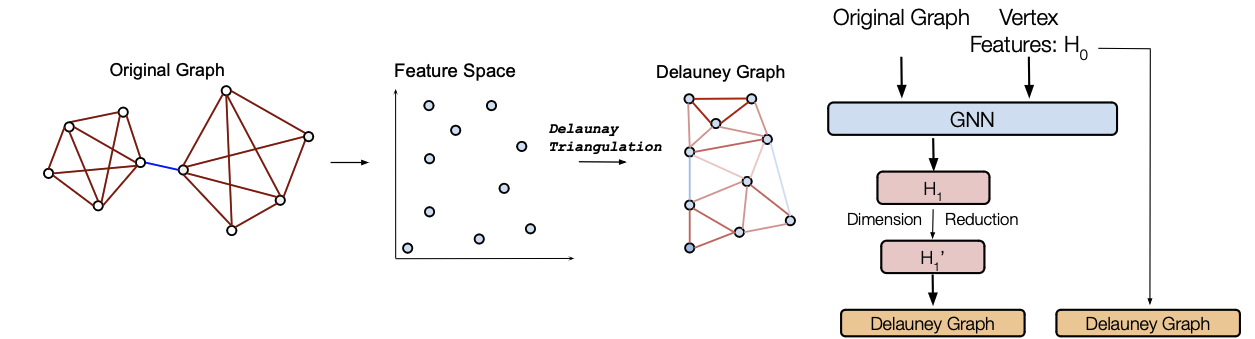
\includegraphics[width=0.6\textwidth]{figures/Delaunay-Rewiring.png}
    %     \caption{Illustration of the Delaunay [Attali al., 2024] \cite{attali2024delaunay}}
    % \end{figure}

\end{frame}

\begin{frame}
    \frametitle{Delaunay Graph properties}
    % TODO
    Sparse graphs

    Raise the homophily value of heterophilic graphs.

    \begin{block}{Reduce over-squashing}
        $\iff$ Reduce the negative curved edges \\$\iff$ maximize triangles + minimize squares.
    \end{block}
    \begin{block}{Reduce over-smoothing}
        Largest cliques limited to 3 nodes $\Rightarrow$ no over-smoothing \cite[Nguyen et al, 2023]{nguyen2023revisiting}.
    \end{block}
\end{frame}
% =====================================
% Experiments
% =====================================
\section{Experimental Evaluation}
\subsection{Methodology}
\begin{frame}
    \frametitle{Methodology}
    Aim  to reproduce as closely as possible the experiments of the authors. 
    \begin{itemize}
        \item Get same datasets, and preprocess them.
        \item Train the models with the same hyperparameters.
        \item Finally, we evaluate the models with the same metrics.
    \end{itemize}

        
\end{frame}

\subsection{Results}
\begin{frame}
    \frametitle{Results}
    \begin{exampleblock}{Text Dataset preparation}
        \begin{itemize}
            \item Text8 (English Wikipedia) processed.
            \item OpenWebText (GPT2 training material) processed in 18 hours.
            \item train/validation/test split according to experimental methodology.
        \end{itemize}
    \end{exampleblock}

    \begin{alertblock}{We were unable to run the models}
        \begin{itemize}
            \item Training impossible on our machines (size of model).
            \item Does not work on Colab (tensorflow numpy2 incompatibilities).
            \item No trained model shared by the authors.
        \end{itemize}
    \end{alertblock}
    
\end{frame}

\subsection{Discussion}
\begin{frame}
    \frametitle{Discussion}
    \textbf{We faced huge challenges}
    \begin{itemize}
        \item Graphs
    \end{itemize} 
    
    \textbf{Future paper that will be explored in the report:}
    \begin{itemize}
        \item \textit{Cayley Graph Propagation} by JJ Wilson, Maya 
        Bechler-Speicher, Petar Veličković \cite{wilson2024cayleygraphpropagation}
    \end{itemize}
\end{frame}

% =====================================
% Conclusion
% =====================================
\section{Conclusion}
\begin{frame}
    \frametitle{Conclusion}
    \begin{itemize}
        \item Cannot confirm the results o
        \item Not able to reproduce.
        \item Hard time digging in code and documentation.
    \end{itemize}

    \begin{block}{Do you have any question?}
        
    \end{block}
\end{frame}

% Automatic bibliography
\begin{frame}[allowframebreaks]
    \frametitle{References}
    \scriptsize
    \bibliography{references}
    \bibliographystyle{plain}

\end{frame}

% =====================================
% Additional slides
% =====================================
\begin{frame}
    \frametitle{Curvature}
    \label{curvature}
    \small
    Balance Forman Curvature \cite[Topping, 2022]{topping2022understandingoversquashingbottlenecksgraphs} is computed over cycles of size 4.
    $$c_{ij}= \frac{2}{d_i} + \frac{2}{d_j} - 2 + 2 \frac{\sharp_{\Delta}}{\max(d_i, d_j)} + 
            \frac{\sharp_{\Delta}}{\min(d_i, d_j)} + 
            \frac{\max(\sharp_{\square}^i,\sharp_{\square}^j)^{-1}}{\max(d_i, d_j)}
            (\sharp_{\square}^i + \sharp_{\square}^j)
    $$

    {\tiny
    where $\sharp_{\Delta}$ is the number of triangles based at $e_{ij}$, 
    $\sharp_{\square}^i$ is the number of 4-cycles based at $e_{ij}$ starting from $i$
    without diagonals inside.
    }

    \begin{columns}
        \begin{column}{0.6\textwidth}
            \begin{block} {Curvature of graph edges}           
            \begin{itemize}
                \small
                \item Positive curvature edges establish connections between 
                nodes belonging to the same community.
                \\Highly positive curved edges $\rightarrow$ over-smoothing \cite[Nguyen et al., 2023]{nguyen2023revisiting}.
                
                \item Negative curvature edges connect nodes from different communities.
                \\Highly negative curved edges $\rightarrow$ over-squashing \cite[Topping et al., 2021]{topping2022understandingoversquashingbottlenecksgraphs}.
            \end{itemize}
        \end{block}

        \end{column}
        \begin{column}{0.4\textwidth}
            \begin{figure}
                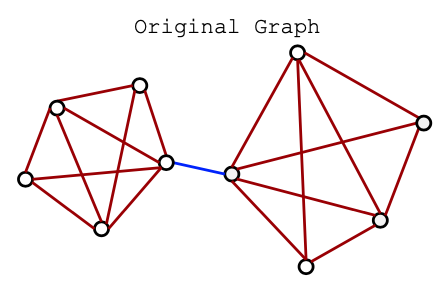
\includegraphics[width=0.9\textwidth]{figures/original_graph.png}
                \caption{\scriptsize Example graph: in red the edges with positive curvature ($\sim 3$), 
                in blue with negative curvature (-1.2) \cite[Attali al., 2024]{attali2024delaunay}}
            \end{figure}
        \end{column}
    \end{columns}
\end{frame}


\begin{frame}
    \frametitle{Delaunay Triangulation}
    \small
    \begin{block}{Definition}
        A Delaunay triangulation, denoted as $DT(P)$, for a set $P$ of points 
        in the $d$-dimensional Euclidean space, is a triangulation where no 
        point in $P$ resides within the circum-hypersphere of any $d$-simplex 
        in $DT(P)$.
        
    \end{block}
    \begin{columns}
        \begin{column}{0.6\textwidth}
        In  two dimensions, Delaunay triangulations maximize the angles of triangles 
        formed by a set of points $\rightarrow$ triangle $\sim$ equilateral.

         
        \emph{Figure: \href{https://shwestrick.github.io/2021/12/18/delaunay-viz.html}{Sam Westrick}}
        \end{column}
        \begin{column}{0.4\textwidth}
            \begin{figure}
                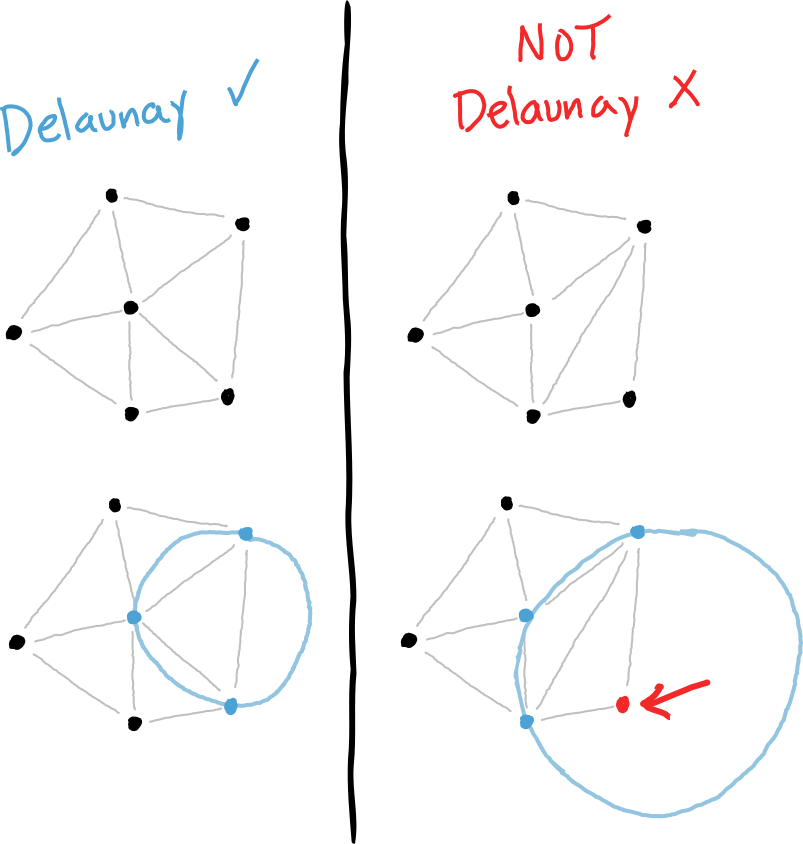
\includegraphics[width=0.7\textwidth]{figures/delaunay-not-delaunay.png}
                
            \end{figure}
        \end{column}
    \end{columns}
\end{frame}

\begin{frame}
    \frametitle{UMAP}
    \small
    Uniform Manifold Approximation and Projection (UMAP) is a dimensionality 
    reduction technique that can be used for visualisation similarly to t-SNE,
    but also for general non-linear dimension reduction.
    UMAP constructs a high dimensional graph representation of the data 
    then optimizes a low-dimensional graph to be as structurally similar as possible.
    \begin{columns}[t]
        \begin{column}{0.6\textwidth}
            \begin{block}{Advantages}
                
                \begin{itemize}
                    \scriptsize
                    \item \textbf{Speed}: UMAP is faster than t-SNE.
                    \item \textbf{Global structure}: UMAP preserves more of the global structure.
                    \item \textbf{Separation}: clearly separate groups of similar categories.
                \end{itemize}
            \end{block}
            Dimensionality reduction technique is perfect - by necessity, we're distorting the data to fit it into lower dimensions - 
            and UMAP is no exception. But it is a powerful tool to visualize and understand large, high-dimensional datasets.
        \end{column}
        \begin{column}{0.4\textwidth}
            \begin{alertblock}{Hyperparameters choice}
                \scriptsize
                Most common: \texttt{n\_neighbors} and \texttt{min\_dist}, control the balance between local and global structure.

            \end{alertblock}
            \begin{figure}
                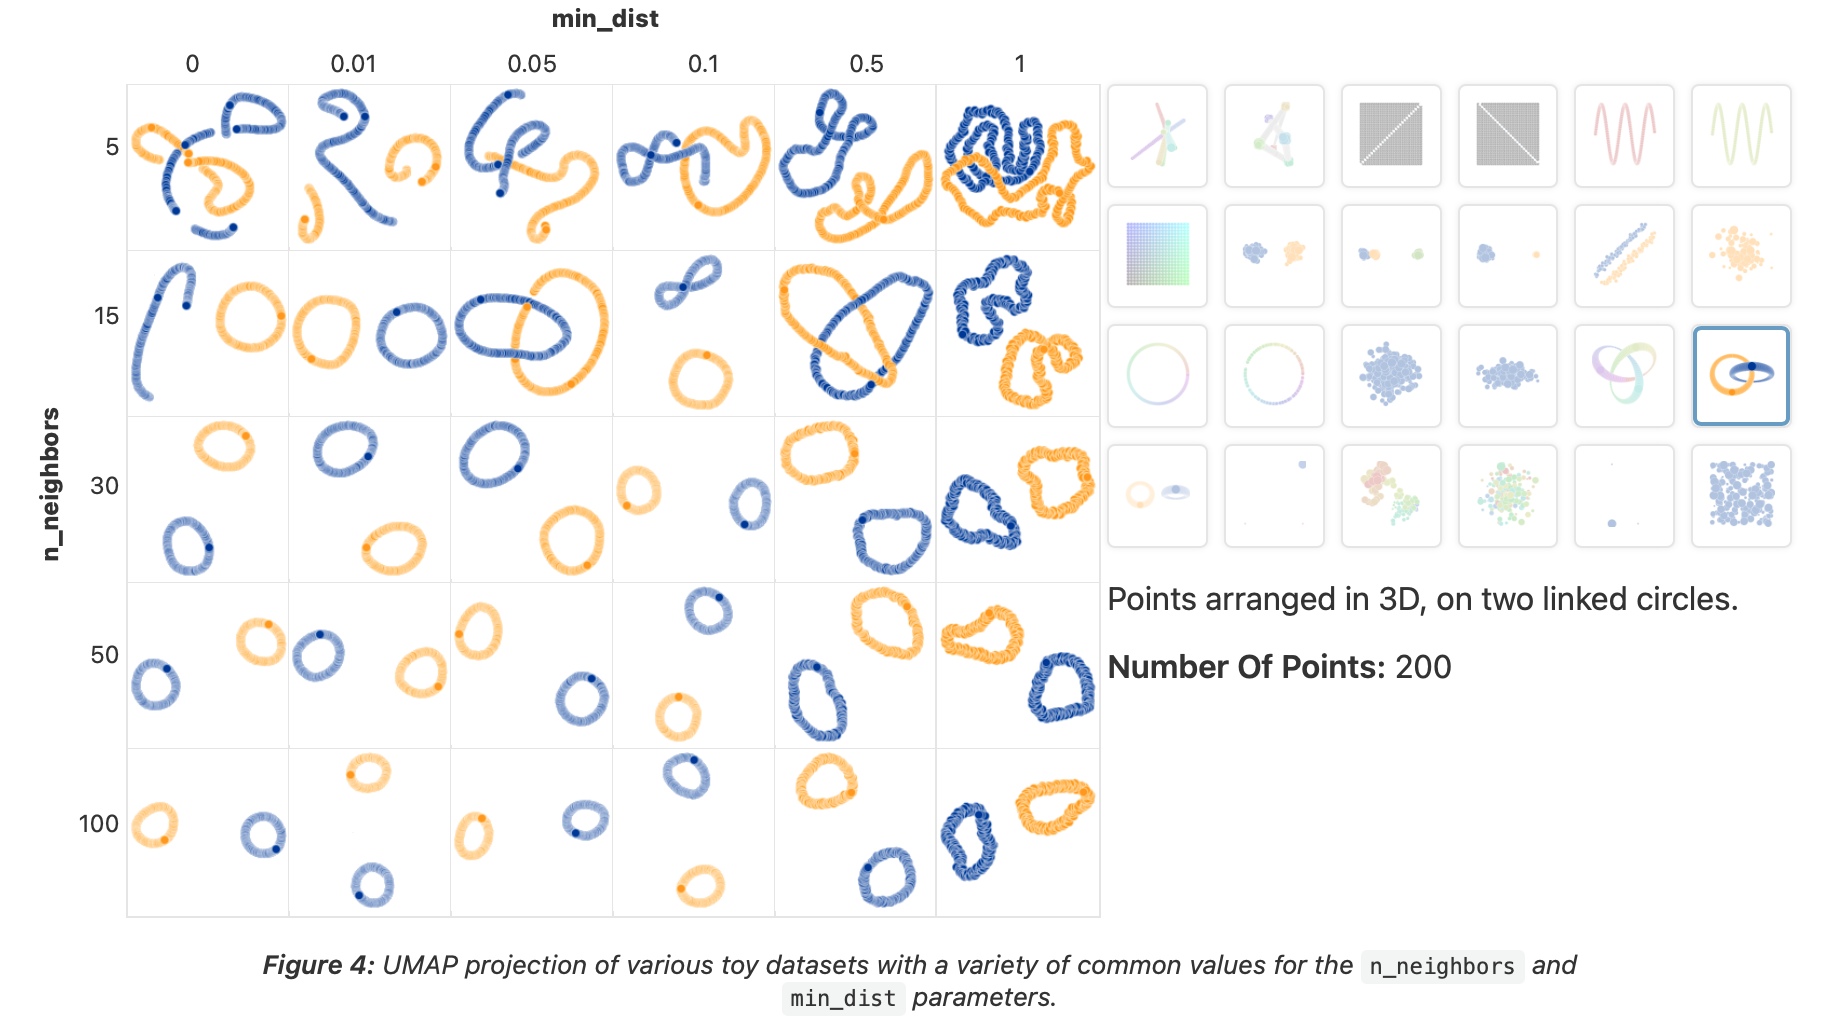
\includegraphics[width=0.8\textwidth]{figures/UMAP_hyperparam.png}
                \caption{\scriptsize Illustration of UMAP hyperparameters from 
                    \href{https://pair-code.github.io/understanding-umap/index.html}{Google PAIR}}
                
            \end{figure}
        \end{column}
    \end{columns}


\end{frame}

\end{document}